\documentclass[a4paper, 12pt]{report}
\usepackage{graphicx} % Required for inserting images
\usepackage{fullpage}
\usepackage{longtable}
\usepackage{caption}
\usepackage{hyperref}
\usepackage{biblatex}
\usepackage{subcaption}
\addbibresource{references.bib}
\usepackage{setspace}
\onehalfspacing
\usepackage{indentfirst}
\setlength{\parindent}{4em}

\usepackage{forloop}
\newcounter{loopctr}
\newcommand{\rpt}[2][1]{ \forloop{loopctr}{0}{\value{loopctr}<#1}{#2} }
\newcommand{\on}[1][1]{\forloop{loopctr}{0}{\value{loopctr}<#1}{&\cellcolor{gray}}}
\newcommand{\off}[1][1]{\forloop{loopctr}{0}{\value{loopctr}<#1}{&}}
\usepackage{xcolor,colortbl}
\usepackage{tabularray}
\usepackage{amssymb}
\usepackage{titlesec}

\titleformat{\chapter}[block]
  {\normalfont\huge\bfseries}{\thechapter\hspace{10pt}}{0pt}{\Huge\bfseries}

\newcounter{originalchapter}
\newcommand{\abstractchapter}[1]{%
  \setcounter{originalchapter}{\value{chapter}}
  \setcounter{chapter}{0}
  \renewcommand{\thechapter}{0}
  \chapter*{0 #1}
  \addcontentsline{toc}{chapter}{0 #1}
  \setcounter{chapter}{\value{originalchapter}}
  \renewcommand{\thechapter}{\arabic{chapter}}
}

\title{\textbf{FoodWhizNet: A Web-based Food Classification System using Multi-Color Space Siamese-CNN Model}}
\author{Samson Jr Rollo}
\date{January 2024}

\begin{document}

\begin{titlepage}
    \centering
    \vspace*{1cm}
    {\LARGE\bfseries FoodWhizNet: A Web-based Food Classification System using Multi-Color Space Siamese-CNN Model \par}
    \vspace{2cm}
    {\Large Samson Jr Rollo \par}
    \vspace{1cm}
   	CMSC 199.1: Research in Computer Science I \\
	Division of Natural Sciences and Mathematics \\
	University of the Philippines Tacloban College\\
	sdrollo@up.edu.ph\\
    \vfill
    January 2024
    \vfill
\end{titlepage}
%\maketitle


\pagenumbering{gobble}
\abstractchapter{Abstract}
\input{chapters/Abstract}
% \chapter*{Dedication}
% \addcontentsline{toc}{section}{Dedication}
% Lorem Ipsum is simply dummy text of the printing and typesetting industry. Lorem Ipsum has been the industry's standard dummy text ever since the 1500s, when an unknown printer took a galley of type and scrambled it to make a type specimen book. It has survived not only five centuries, but also the leap into electronic typesetting, remaining essentially unchanged. It was popularised in the 1960s with the release of Letraset sheets containing Lorem Ipsum passages, and more recently with desktop publishing software like Aldus PageMaker including versions of Lorem Ipsum.
% \chapter*{Acknowledgement}
% \addcontentsline{toc}{section}{Acknowledgement}
% Lorem Ipsum is simply dummy text of the printing and typesetting industry. Lorem Ipsum has been the industry's standard dummy text ever since the 1500s, when an unknown printer took a galley of type and scrambled it to make a type specimen book. It has survived not only five centuries, but also the leap into electronic typesetting, remaining essentially unchanged. It was popularised in the 1960s with the release of Letraset sheets containing Lorem Ipsum passages, and more recently with desktop publishing software like Aldus PageMaker including versions of Lorem Ipsum.

\tableofcontents
\addtocontents{toc}{\protect\thispagestyle{empty}}

\newpage

\pagenumbering{arabic}
\chapter{Introduction}
Food is essential to humans in order to survive, situated at the bottom of the hierarchy of needs by Maslow \cite{Mcleod2023} together with shelter and clothes. The task of classifying them accordingly benefits not only personal gain but also the professional field, for instance, the medical science and nutrition field where multiple uses include diet planning \cite{chun-2022, de-kervenoael-2023,zhou-2019}. It is becoming one of the wake-up calls for most people to live a healthy lifestyle after the COVID-19 pandemic. Being able to know what food you are eating is the best way to start living healthy. Classifying the foods you are eating is sometimes not an easy task especially since there are plenty of foods available worldwide. Food classification does not stop on personal use only. The science community benefits from this also as this becomes a way for most improvements to models and algorithms in various problems, for instance in classification problems.

With the rise of Artificial Intelligence and the Internet of Things marking the fourth industrial revolution \cite{sarker-2021}, the aim to automate food classification is also popularized. With the advent of Deep Learning and its variant architectures such as Convolutional Neural Networks \cite{lecun-2015,shrestha-2019} comes with the task of creating a robust and effective model to cater to the needs of going together in the tides of technology.

To utilize the power of deep learning, this study aims to create a robust and effective model that utilizes multiple variations of a single feature, the color, to be fed on a Siamese CNN model pre-trained with EfficientNetB0. Thus, this study is titled \textit{FoodWhizNet: A Web-based Food Classification System using Multi-Color Space Siamese-CNN Model}.

This paper is organized accordingly. Part 1 is the Introduction containing Section 1.1 which provides a background of the study together with the terms and concepts relevant to the food image classification problem. Part 2 provides an elaborate review of related literature. Part 3 indicates the research gap and problem that this study aims to address. Part 4 defines both the general and specific objectives of the study. Part 5 for the scope and limitation, Part 6 covers the significance of the study, and Part 7 addresses both the theoretical and conceptual frameworks. Part 8 focuses on the discussion of the proposed tools and methods. Part 9 provides the initial gathered results from the initial experiments. Part 10 highlights schedule of activities for this study.  
\section{Background of the Study}
\subsection{Food Classification}
Food classification can have its benefits to either professional sectors or for personal gain. May it be for creating a diet plan for a healthy lifestyle or may it be for traveling abroad to familiarize yourself with novel foods. In consideration of the number of food classes around the world, the complexity to which a single food can be classified also increases. This is because the food classification problem has a unique characteristic for it to be a difficult task to go with. This is its high and low intra-class variability \cite{ciocca-2019} and non-linearity \cite{islam-2018} so classifying food class accordingly always came with a caveat. In the conduct of various studies with regards to food classification, some of the most common datasets include the Food-101 \cite{bossard-2014}, UECFood100 \cite{matsuda-2012}, and UECFood256 \cite{kawano-2014,kawano-2015}. These datasets were also used for benchmarking the models created from either machine learning or deep learning. Other studies conducted on food classification create their dataset such as that of \cite{pandey-2017} for localization of the learned model.
\subsection{Deep Learning and CNN}
As artificial intelligence advances, new fields are being unlocked to address the weaknesses of the current fields. The introduction of deep learning as a subset of machine learning gave way to a more sophisticated yet robust way of learning things without almost human intervention in the preparation of data. Deep learning as mentioned in Lecun et al. \cite{lecun-2015} is a way to make models learn the features and representation of the input on their own by conducting its own feature extraction and analyzing the representation through the multiple layers of the model with minimal external intervention. The conception of deep learning has also brought to us the robustness and increase in productivity as well as the accuracy of the task to be conducted. Shrestha and Mahmood \cite{shrestha-2019} conducted a review on deep learning and its architecture. Deep learning architectures include deep residual networks, reinforcement learning, deep convolution networks, autoenconders, and more. This study will be utilizing a Convolutional Neural Network or CNN due to its appropriateness to image classification \cite{sarker-2021} so it will be mentioned more. CNN is one of the most common architectures of the Deep Neural Network (DNN) that utilizes multiple layers of representation and concatenates the layer output at the end to have a defined output. As part of the DNN, CNN also faces two major challenges such as overfitting, premature convergence, vanishing gradient, exploding gradient, training time, and more \cite{shrestha-2019}. In order to address these issues, one should be aware of these challenges and the set of solutions provided as well as the use of appropriate parameters for the model.
\subsection{Siamese Convolutional Neural Networks}
Siamese Convolutional Neural Network or SCNN is a variation of CNN that contains two identical sub-networks \cite{prasad-2021}. The sub-networks have similar parameters and architecture. This particular type of CNN is best used for checking the similarity or dissimilarity of two inputs. Due to its robust characteristic of classifying similarity between two images, it is effective in steganalysis \cite{you-2021}. SCNN is also best used with fingerprint matching and face verification tasks. SCNN application on food classification can also be seen in \cite{sarker-2019} where the one-shot learning was exploited. In this study, SCNN will be utilized to record the similarity index of the spectral feature extracted from the food image. The structure of Siamese CNN also inspired some of the Multiple layered CNN pipelines such as \cite{martinel-2018, pandey-2017}.
\subsection{Pre-trained CNN Models}
Pre-trained CNN models are those models that have already undergone the process of training and already have defined weights. Yalcin \cite{yalcn-2021} discussed the notion of transfer learning and its uses. Basically, transfer learning uses pre-trained models to alleviate the costly training process of novel or similar models. Existing models such as VGG-19 \cite{simonyan2015deep} used for image classification problems \cite{bansal-2021} was a 19-layer deep CNN trained using an ImageNet database with more than a million images and over 140M parameters. This model was trained using 224 x 224 image dimensions and can classify for up to a thousand classes. Another pre-trained model is the InceptionV3 \cite{Szegedy_2015_CVPR} which was developed by Google and was also trained using the ImageNet with an image dimension of 299 x 299 and over 20M parameters. It has a depth of about 50 layers and can classify up to a thousand classes. ResNet50 \cite{He_2016_CVPR} or the Residual Network is also one of the pre-trained models used for transfer learning. It was also trained using the ImageNet database with over a million 224 x 224 sized images with a depth of 50 layers and over 20M parameters. This too can classify over a thousand classes. Another popular pre-trained model is the EfficientNet \cite{pmlr-v97-tan19a} which has 8 variations (from B0 to B7). Even the simplest B0, having over 5M parameters can achieve satisfactory accuracy, whereas B7 has over 60M parameters with greater accuracy compared to other pre-trained models at such low parameters. MobileNet \cite{howard2017mobilenets} being the smallest pre-trained model with 4M parameters on its baseline and 3M parameters on its V2 and a depth for both of 88 layers. Despite its small size, it can still satisfactorily classify objects, perfect for conducting initial experiments on novel or hybrid models.
\subsection{Multi-Color Space}
The importance of color can be related to its effect on the sense of sight as according to Fries \cite{grusser-1989}, the sense of sight is the window that takes us beyond and apprehends everything that our sight could perceive including colors. Its importance is not limited to humans alone but it also creates a huge impact in the image analysis carried out by artificial intelligence, such as that of deep learning \cite{larbi-2018,he-2019,hirota-2020}. Its utilization as a spectral feature for deep learning such as in \cite{al-sarayreh-2018} can result in a satisfactory accuracy but not better than other features, or combinations as such. To address the satisfactory performance of using single colors in conducting image analysis, the use of multiple color spaces as input can be utilized as different color spaces correspond to different conditions such as lighting and noise. There are already studies in relation to the use of multiple color spaces, one is from Gowda and Yuan \cite{gowda-2019} which suggests that there is a right color space for certain image classes and that combination of certain color spaces can improve accuracy for certain image analysis problem. The most common color space that is utilized for most image classification problems is the RGB which contains the Red, Green, and Blue color channels. Each channel has values ranging from 0 to 255. Machine Learning defaults to the use of RGB color space unless specific tasks require other color space to be used.  Another commonly used color space is the HSV which contains the Hue, Saturation, and Value channels. Its channel has values ranging from 0 to 360 for Hue, and 0 to 100 for both Saturation and Value channels. HSV is useful in image identification as it can segment better the objects in an image \cite{sural-2003}. More color spaces exist like the LAB which is based on the Lightness and RGBY colors, the YPbPr, YCbCr, YDbDr, YUV, XYZ, etc.
\chapter{Related Works}
There has been already a wide variety of food classification studies that utilized various features and models. It is in this chapter that these related works of literature are reviewed about the proposed study. This chapter will include pieces of literature about existing food classification systems with deep learning and color spaces. 

%food classification, siamese, and cnn rrl
Zhou et al.\cite{zhou-2019} provide a review of several studies that utilized deep learning in food classification problems. It also includes a discussion about deep learning and its conception of food classification analysis. He concluded that there is a huge impact on the introduction of deep learning to food research because it revolutionizes as well as produces a robust and accurate approach to food classification. Despite the challenges that food classification can pose such as that presented by Ciocca et al. \cite{ciocca-2019} that food analysis is a difficult task due to the intrinsic high and low intra-class variability of the food segment. 

Focusing on the literature related to the food classification system, Vijayakumari et al. \cite{vijayakumari-2022} and Islam et al. \cite{islam-2018} focus on the use of transfer learning of a single CNN. Particularly \cite{vijayakumari-2022} utilized the EfficientNetB0 model and transformed it into a problem-dependent model based on the Food101 \cite{bossard-2014} dataset. While \cite{islam-2018} utilized the Inception V3 base model for transfer learning using the Food-11. Transfer learning freezes most of the layers except the top layer. This utilizes the pre-trained weights that the model has. In the case of these two studies, they were based on the ImageNet. This can be very helpful if the input image does not undergo color space conversion considering the the pretrained weights were in RGB therefore the problem-dependent task matches the problem-independent requirements. 

In Vijayakumari et al. \cite{vijayakumari-2022} conduct of study, they have proposed the use of EfficientNetB0 as a source for their transfer learning. Starting from the problem-independent pre-trained model EfficientNetB0, they have extended the model by adding their problem-dependent network used for fine-tuning EffiecientNetB0's feature maps. The structure is similar to the naive CNN with another set of networks connected after each pooling layer. Also, they noted that the use of a rectified linear unit was in effect for the nonlinear activation operation. The proposed model consists of four methods, all have the EfficientNetB0 as the CNN, input size of 224x224, data augmentation technique of horizontal flipping and rotation, pooling using the global average pooling 2d, loss function of categorical cross-entropy, and ran a 100 epoch. Model 3 and 4 has a mixed float 16 for the mixed precision parameter. Models 1 and 3 have a learning rate of 1e\textsuperscript{-2}, while Models 2 and 4 have a learning rate of 1e\textsuperscript{-4}. They have used the Food-101 dataset \cite{bossard-2014} with a 75-25 train-test split. The results were analyzed according to the precision, recall, and f1-score. Among their four proposed methods, Model 4 has the highest score with more than 80\% across all three metrics. They have also surpassed their predecessor's accuracy. 

Another transfer learning study on food classification that was mentioned was on Islam et al. \cite{islam-2018}. Recognizing the challenging task of the food classification problem due to its non-linearity, they have proposed a CNN model using transfer learning with Inception V3 which is pre-trained with ImageNet. To address their hardware resource limitation, they have used the Food-11 dataset which contains 16643 images with 11 classes. In their experimental setup, they utilized an 80-10-10 train-validation-test split. The same with most image classification systems, they have conducted image preprocessing to lessen the training time. Specific to their experiment is the use of the ZCA whitening reduction method which reduces the redundant image pixels to emphasize more the features of the image. They have also set the dimension of the input image specific to the model they are using, the 299 x 299 x 3 dimension. The result of the study shows a staggering 92.86\%, outperforming fine-tuned AlexNet by 10.63\% and CaffeNet by 12.84\%.

An additional food classification system approach is the use of multiple parallel Convolutional Neural Networks. The study of Pandey et al \cite{pandey-2017}, Martinel et al. \cite{martinel-2018}, and Al-Sarayreh et al. \cite{al-sarayreh-2018} utilized the power of different base models ran in parallel to exploit its strength to mine discriminative features. These parallel CNNs are not necessarily the same since they want to make the best out of a particular pre-trained model. For instance, Martinel et al. \cite{martinel-2018}, have used two networks in parallel, one is a pre-trained ResNet to capture all the generic features and one is for capturing the vertical features of food images. The use of multiple parallel CNNs has shown its efficient performance in classification tasks. Moreover, another set of studies that focuses on the use of multiple parallel CNNs is that of fake image detection tasks such as He et al. \cite{he-2019} and Larbi et al. \cite{larbi-2018}.

Expounding Pandey et al.\cite{pandey-2017}, a food classification system was developed to address its predecessors' accuracy and robustness concerns while considering the intra-class variability characteristic of the food classification problem. By utilizing both the Food-101 dataset\cite{bossard-2014} and a novel Indian food dataset, they have proposed to create an ensemble of multiple layered CNN pipelines. Using AlexNet as the baseline architecture for the proposed model and the Siamese CNN structure, they have devised a 3-layered pipeline with AlexNet, GoogleNet, and ResNet as its sub-networks. The authors believed that each of the sub-network's best characteristics would contribute to better classification accuracy. Similar to most image classification systems, images are first preprocessed to be fed to the model. For the Food-101 dataset, RGB images were first converted to HSV for proper histogram equalization before converting back to RGB for processing. They have set the maximum side length to 512 pixels and used the 75-25 train-test split. A different approach was done on the local dataset where minimum size was ensured and no maximum size was enforced. They also used 80-20 train-test splits for this particular dataset. They have conducted their experiments using handcrafted features and CNN feature descriptors. The study produced a promising output with 73.50\%, 94.40\%, and 97.60\% for Top-1\%, Top-5\%, and Top-10\%, respectively on the Indian food dataset which is much higher than each of the individual sub-network's accuracy. It also has a higher accuracy using the Food-101 dataset with 72.12\%, 91.61\%, and 95.95\% for Top-1\%, Top-5\%, and Top-10\%, respectively.

%martinel, 2018
Also in Martinel et al. \cite{martinel-2018} a novel approach was developed to food recognition using a combination of slice network with slice convolution layer and residual network. This study is included in the review since it includes food classification. One of the networks is the wide residual network which is a pre-trained model through ImageNet 2012 and the other is the slice network which is in naive implementation from scratch, proposing the WISeR model, a combination of the two sub-networks. Their slice sub-network was used to capture and exploit the vertical features of the food images because one of their hypothesis was that many of the dishes from the dataset are characterized by so. In the wide residual sub-network, they have followed the use of a series of batch normalization and rectified linear units for preactivation for their CNN as well as increasing their feature map size as it progresses along the sub-network addressing the diminishing feature problem and capturing the rest of the generic features that haven't been captured by the slice sub-network. The datasets used were the UECFood100 \cite{matsuda-2012}, UECFood256 \cite{kawano-2014,kawano-2015}, and Food-101 dataset \cite{bossard-2014}. In their Food-101 dataset, the 75-25 train-test split was used. They have evened out the learning rate for the slice sub-network to match it with the existing units created by the wide residual sub-network, as well as fine-tuning the model by taking 224 x 224 images and conducting data augmentation techniques such as horizontal flipping, aspect ratio augmentation, photometric distortions, and alexNet-style color augmentations. Running a total of 100k iterations with an initial learning rate of 0.01 updating to 0.002 after 50k iterations to 0.0004 after 90k iterations with constant weight decay of 0.0005 and 0.9 momentum for all layers.  Overall, the proposed WISeR model outperforms the existing models in the food recognition problem, resulting in 90.27\% Top-1\% and 98.71\% for the Top-5\%. Their study also found that the use of the pre-trained model outperforms new models supporting the claim of Vijayakumari et al.\cite{vijayakumari-2022}. This was done on their ablation analysis on each sub-network. For the three datasets, the wide residual network outperforms the slice convolution network.

Another study on multiple parallel CNN and spectral input is Al-Sarayreh et al. \cite{al-sarayreh-2018} who conducted a study on red-meat adulteration using spectral and spatial features. Using hyperspectral imaging, they extracted their dataset from collected meat from various sources as a hyperspectral cube with dimensions \textit{w} x \textit{l} x \textit{g}, where \textit{w} is the width, \textit{l} is the length, and \textit{g} is the intensity of the reflected light. With 75 samples, the study follows a 76-24 train-test split with six calibrations, four sets of collected samples, and three classes. The calibrations were fresh red meat unpacked, freshly packed, frozen unpacked, frozen packed, frozen-thawed unpacked, and the ground truth. The four samples were lamb, beef, pork, and fat. The samples are divided into three classes, LAMB class for lamb samples, FAT class for fat samples, and OTHER class for beef and pork samples. The proposed model has the same structure as the Siamese CNN but has an unbalanced sub-networks. Since they take two inputs, the spectral and spatial features, each input is processed differently, such that spectral input is fed to a 1D CNN utilizing the mean spectrum extracted from the HSI using the Kennard-Stone algorithm when sampling the superpixels. Superpixels were generated using the SLIC superpixel algorithm. They have noted that to have the spatial feature input which was fed on a 3D CNN, they have used PCA space over the SLIC superpixel to match the spectral input. They have also conducted a preprocessing of the spectral input by utilizing the Savitsky-Golay algorithm to normalize it by smoothing and de-spiking. The proposed model was trained using forward propagation and back propagation. For each layer, the output feature is concatenated and undergoes the same process until the very end where the output is defined using the softmax activation function. For the back propagation, stochastic gradient descent was used with a categorical focal loss function. To address the overfitting issue, they have enforced regularization and dropout techniques. The setup was given by running 500 epochs with a 0.003 learning rate, momentum of 0.9, and a rectified linear unit on the hidden layers. Overall, they analyzed the experiment using the f1-score and overall accuracy. Outperforming the conventional SVM spectral-based and SVM spatial-based models, at 94.4\% accuracy. Although performing last among the three, the SVM spectral-based model still achieves an overall accuracy of 91.4\%.

To discuss the use of multiple color space input, related studies are also presented such as in Larbi et al. \cite{larbi-2018} who conducted a study on the efficiency of using multi-color CNN on Face Spoofing detection. The same goes with He et al.\cite{he-2019} where the use of multiple color spaces on the GAN-generated images was used. Furthermore, Gowda and Yuan \cite{gowda-2019} test the effectiveness of using different color spaces on image classification using the CIFAR dataset.

In Larbi et al. \cite{larbi-2018}, they used the three color spaces; RGB, HSV, and YCbCr, as an input to each of the three identical CNN models. The selection process was done using a voting mechanism. The extraction sequence of the color space affects the generation of histograms therefore creating a noticeable difference between the real and fake face.

Moreover, He et al. \cite{he-2019} also conducted a study on fake image detection made by GAN techniques using CNN with an RF ensemble. They focused mainly on the use of chrominance components from HSV, YCbCr, and Lab for robust detection in detecting fake images. Similar to \cite{larbi-2018}, the proposed methodology utilized three identical CNNs but differed in the input for each model, and the depth of the model. It was mentioned that YCbCr is good for lossy compression of digital images, and HSV is best applied on computer vision tasks.

Gowda and Yuan \cite{gowda-2019} investigated the importance of color spaces in image classification. Their study opened a new challenge to the current study concerning data profiling. They mentioned the existence of sRGB from the CIFAR dataset which may affect the feature extraction of the proposed study if any images have the same image format from the Food-101 dataset \cite{bossard-2014}. Additionally, they have mentioned some of the popular color spaces including HSV, lab, YUV, YCbCr, XYZ, YIQ, HED, LCH, and CMYK. For which combining color spaces can increase the accuracy of image classification algorithms. They also reasoned out that certain color space is appropriate to certain classification problems.  In consideration of the two-input model, their study produced a table where the combination of YUV and LAB color spaces produced the highest accuracy from their selected color spaces on the CIFAR-10 dataset with a simple CNN model. The use of LCH, YPbPr, and XYZ color spaces degraded the overall accuracy of their model, therefore discarding it. The use of RGB, YIQ, LAB, HSV, YUV, YCbCr, and HED were recommended to produce high accuracy in image classification problems.

In support of the previously reviewed study, Kang \cite{kang-2011} also suggested the use of CIELab or LAB color space in evaluating food images. The ability of LAB color space to detect color changes and differences is attributed to its absolute measurement, therefore disregarding any lighting effect on the image. Markovic \cite{markovic2013color} also suggested the use of LAB and RGB color space combinations in food quality evaluation. 

% conclusion
 In relation to the currently proposed study, similarities can be seen from the reviewed works of literature. In consideration of the use of multiple inputs, \cite{al-sarayreh-2018, martinel-2018, pandey-2017} has paved the way by introducing multilayered CNN pipelines with different sub-networks. The only difference is that instead of deviating from the Siamese structure, this study will be using the Siamese CNN as a baseline conforming to balanced sub-networks. The utilization of pre-trained models was also considered since from the reviews, they have a huge impact on the accuracy such that on the study of \cite{al-sarayreh-2018,martinel-2018,vijayakumari-2022}. The effectiveness and high accuracy of the spectral feature \cite{al-sarayreh-2018} of the image such as the color as an input to deep learning also drive the use of color spaces as the primary input to the proposed study. In order to address the need for multiple inputs such as in Siamese CNN, a variety of color spaces is utilized and the selection of color will solely be based on the literature, focusing on a combination of LAB color space and others. 
\chapter{Statement of the Problem}
Food is essential to human survival as per Maslow’s Hierarchy of Needs \cite{Mcleod2023}. It sits at the very bottom of the hierarchy identified as a physiological need together with shelter, water, and clothing. Its heavy significance to humans creates a series of research that revolves mostly around its use, identification, and classification. One of the main research fields that can be related to food is the food classification problem. This is a sub-variant of the image classification problem where machines are taught to classify a certain food to either of the list of classes. This has a practical and beneficial application in various fields not limited to medicine, research, and the restaurant industry. For instance, the use of an image classification system in diet planning can be seen in \cite{brintha-2022,chun-2022,dong2019diet,de-kervenoael-2023}. 

In the food review with the application of deep learning of Zhou et al. \cite{zhou-2019}, most of the models that were developed focus on the conventional features that are present in the food images. Most models that were also developed for food classification systems are either using the naive single feature input CNN, or multiple feature input CNN. Features like color, shape, volume, composition, and texture. One of the distinguished studies was that of Al-Sarayreh et al. \cite{al-sarayreh-2018} which utilized both spectral and spatial features for its meat quality analysis using two unbalanced sub-networks of CNN. The same goes with Pandey et al. \cite{pandey-2017} and Martinel et al. \cite{martinel-2018} which can be generalized to a multilayered CNN pipeline. Using these premises we can arrive at classifying our research problem through our gap. That is the absence of the use of multiple variations of a single input using a balanced sub-network CNN, specifically the multiple color space input. We consider the use of the color feature as an input since it is the most distinguished among the features and multiple studies on multiple color space input for deep learning were also present.

In line with conducting a state-of-the-art alternative approach to classifying food images, the use of the Siamese CNN network model is considered to address the borderline capability of training, testing, and deploying the proposed web-based application. Utilizing a supervised deep-learning network such as CNN is best for this study as this is a sub-variant of the image classification problem \cite{sarker-2021}. To address the multiple variations from a single input, this study will be utilizing Siamese CNN, a specialized type of neural network that best works in similarity and dissimilarity problems that takes two inputs fed on two balanced sub-networks.

The proposed study aims to reach at least the existing best results which uses conventional CNN with inputs used to maximize the utilization of the previously mentioned features. 
\chapter{Objectives}
This section presents the objectives of the study.
\section{General Objective}
To deploy a functional web-based food classification system that utilize multiple color spaces extracted from an image as an input to a Siamese-CNN deep learning network.
\section{Specific Objectives}
\begin{enumerate}
    \item To develop an alternative approach to food classification using multiple color spaces extracted from a food image.
    \item To conduct an ablation study on the best 2-color space input combination for the Siamese-CNN model.
    \item To compare the performance of the proposed model with the current state-of-the-art models in the food classification problem. 
    \item To implement a Siamese-CNN deep learning model on food classification using a web-based application.
\end{enumerate}
\chapter{Scope and Limitations}
The scope of this study is on the development of a food classification system that utilizes a multiple-color space input to a Siamese-CNN deep learning network to be trained and tested using all the classes from the Food-101 dataset \cite{bossard-2014}. The Food-101 dataset will also serve as the primary dataset for this study, utilizing other existing datasets for benchmarking against the previous studies.

For benchmarking purposes, the study will not be utilizing data augmentation techniques to balance the imbalanced datasets. The use of data augmentation technique will be utilized purely to increase the robustness of the proposed model.  

Since this study is training foods primarily found from the Food-101 dataset, the researcher will assume that the user of the web application is querying food classes only included from the Food-101 dataset. Therefore, if any food classes not included in the 101 classes of the primary dataset are queried, they will be categorized to their closest class, disregarding the existence of negative classes.
\chapter{Significance of the Study}
The significance of this study will be associated with the importance of food classification in our everyday life. May it be for professional use in the medical and research field or just for personal use of personal diet plans. Studies that mostly use food classification systems are those that concern the diet of patients with allergies or diabetes for instance. Despite its popularity in the latter fields, the solutions to the food classification problem do not always settle on surface-level use but also for conducting state-of-the-art studies that contribute to the body of knowledge. This is because of the problem's intrinsic high and low intra-class variability characteristics \cite{ciocca-2019}, as well as non-linearity \cite{islam-2018}. Therefore, it is the best avenue for conducting the feasibility of novel and hybrid solutions, especially on a multiple variation single input like the multi-color space input. Since the study explores an alternative way of solving this kind of problem, the choice of using the multi-color space as input is considered. This is to validate the claim of Gowda \& Yuan \cite{gowda-2019} on the effectiveness of using multiple color spaces in the image classification problem, only in our case, applied to the food classification problem. Addressing this gap can spurt future studies on the sole use of multi-color space in image classification problems. In addition to the use of multiple color spaces, the use of Siamese CNN as a model for this study justifies the use of the input. Siamese CNN is known for its robustness in checking for similarity and dissimilarity of two input images, modifying it to learn specific similarities between the color spaces of an image can produce a state-of-the-art study that can also revolutionize deep learning using novel and hybrid techniques. The outcome of this study can be used to validate existing studies as well as create a new node for food image classification on different feature inputs. The deployment of the web-based application will be also utilized in fields not limited to the restaurant industry, medicine, food technology, etc.
\chapter{Theoritical and Conceptual Framework}
Figure \ref{fig:scnn-fc} shows the conceptual and theoretical framework to be used in the study. A dataset is first obtained for the study, specifically a food dataset coming from the Food-101 database \cite{bossard-2014}. The dataset is composed of 101000 food images classified into 101 classifications. The huge amount of samples justifies the use of a deep learning model. After gathering the data needed for the study, it will be split into the train and test sets, specifically, using the 75-25 percent split for the training and testing phase, respectively. All of the instances from both sets will be subjected to resizing, specifically to a 224 x 224 size since this is the required size of the model. After that, each instance will be converted into two color spaces specified in the experiment. This is such that for each sample, two color spaces are generated, for instance, image A is converted into HSV and LAB color spaces. After the conversion, each converted instance is rescaled to [0, 255] value range and then normalized to [0,1]. The normalized instance is again converted to the [0, 255] value range since this is the required input for our model. Additional data augmentation techniques are also applied for the model to be more robust and effective. The data augmentation is only triggered in the training phase of the model. The train set output of preprocessing the inputs can now be fed into the proposed model. The proposed structure is a Siamese CNN network with a pre-trained EfficientNet model, such as EfficientNetB0. The proposed model is fine-tuned to adapt to the food image classification problem. In the training phase, two different color space inputs are required for the Siamese network. An Adam optimizer will be used as well as a categorical focal loss loss function. After the training, the trained model will now be subjected to testing using the test set taken from the dataset. The same with the training phase, the testing phase will also require two color space inputs and will undergo the same preprocessing except for the data augmentation technique. The testing phase will measure the Top-1\% and Top-5\% accuracy. This will help in performing a comparison of the proposed model as well as models from the related studies. Finally, if the best model is achieved, it will be implemented on a web-based application to be deployed for real-world applications.
\begin{figure}[h]
 	\centering
	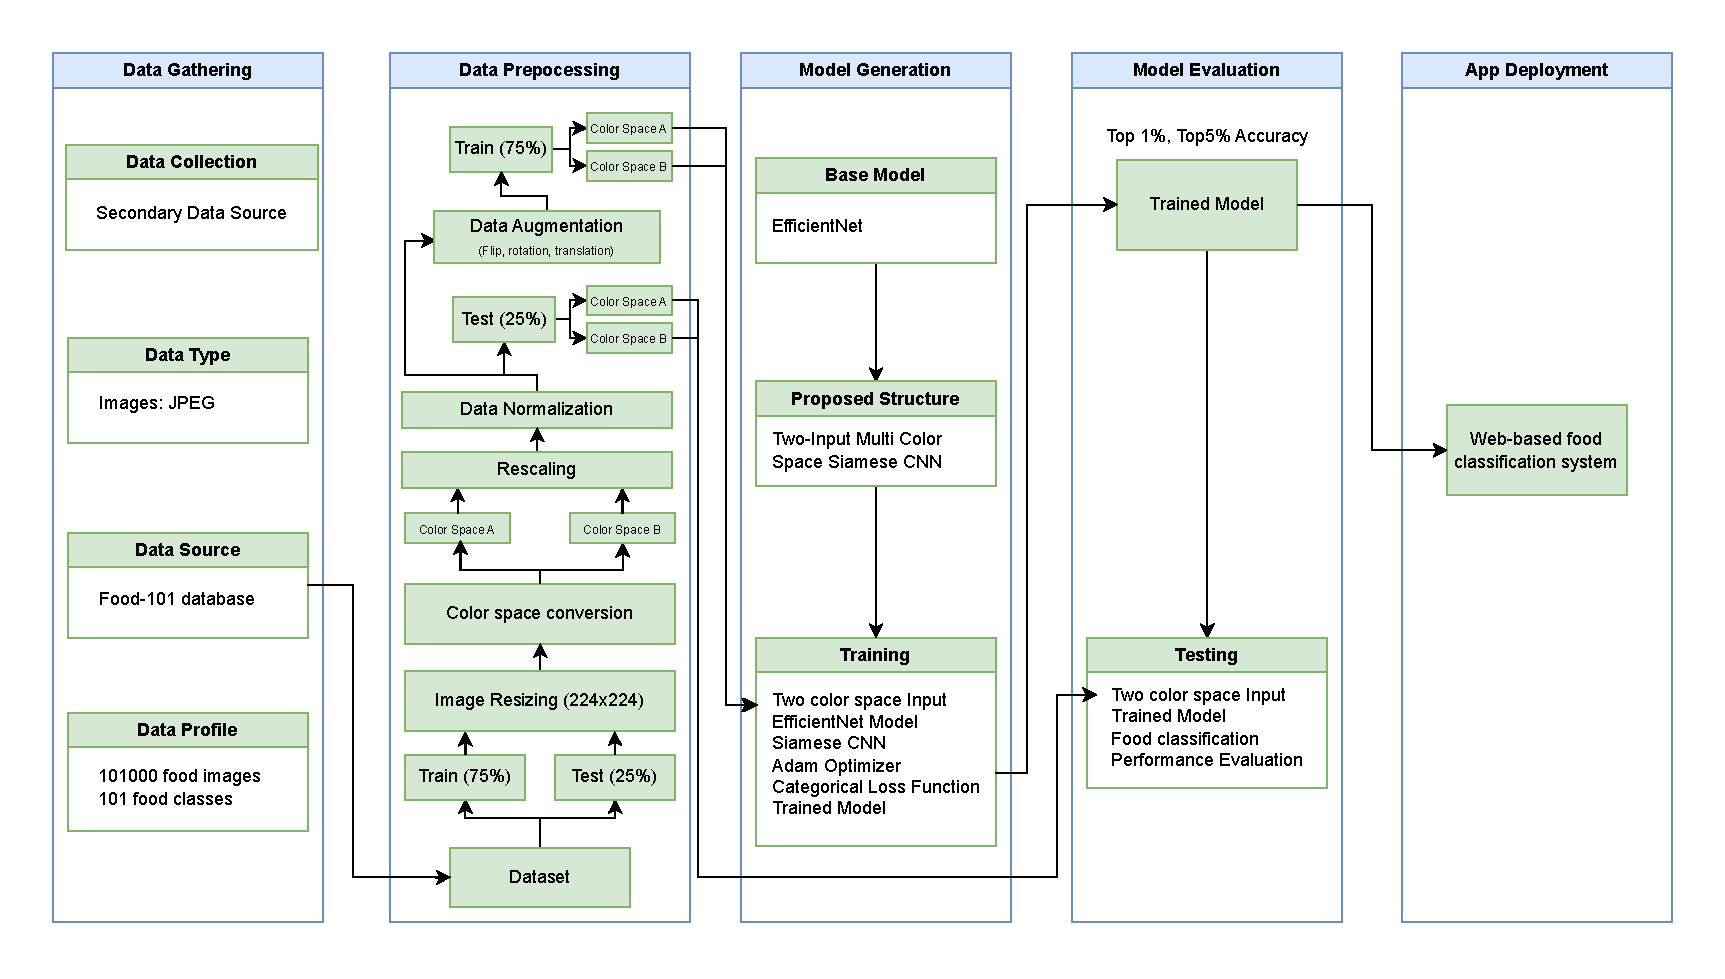
\includegraphics[width=1.15\textwidth]{graphics/images/scnn-fc-concept.pdf}
	\caption{Theoretical and Conceptual Framework}
	\label{fig:scnn-fc}
\end{figure}
\chapter{Proposed Methodology}
\section{Network Design and Architecture}
\begin{figure}[h]
	\centering
	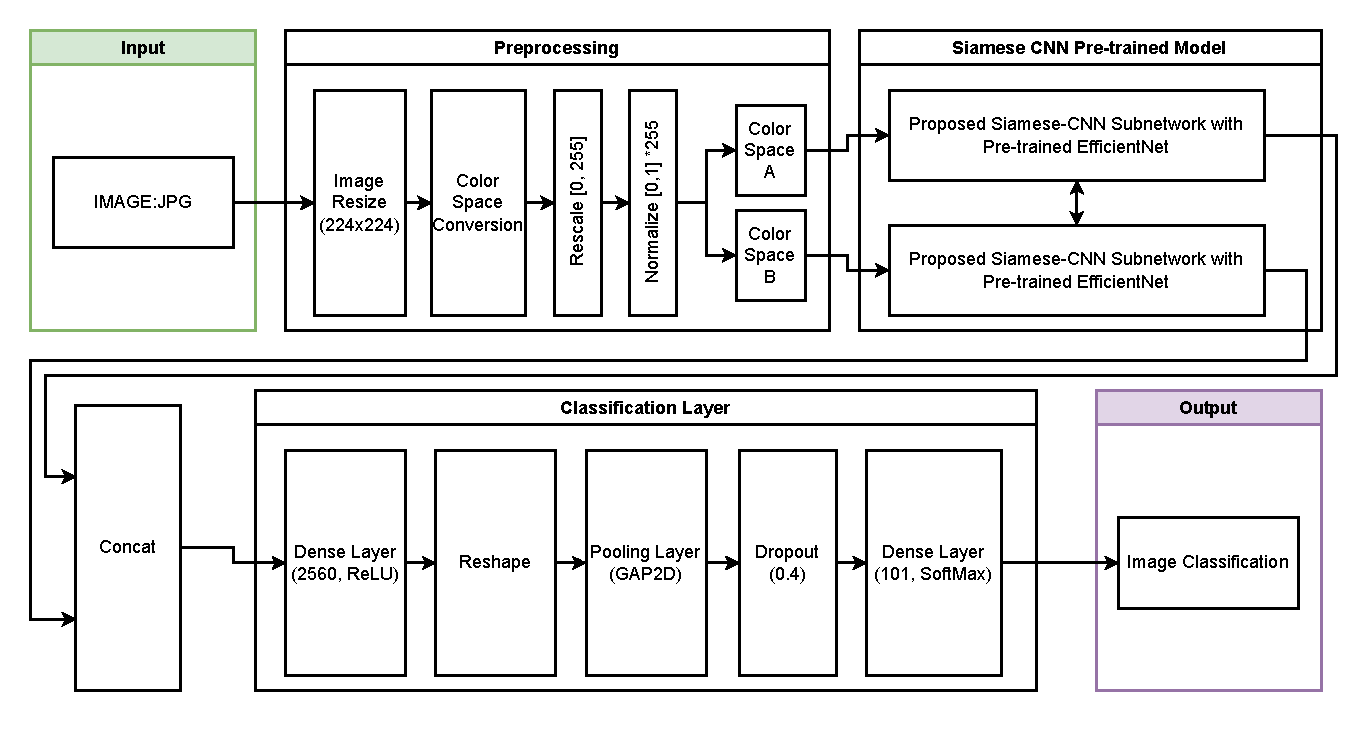
\includegraphics[width=1.0\textwidth]{graphics/images/Proposed_Model.pdf}
	\caption{FoodWhizNet Framework}
	\label{fig:proposedmodel}
\end{figure}

The proposed model will utilize the EfficientNet model family to be fine-tuned to specifically adapt the food image classification problem. This particular model family focuses on balancing the network resolution, width, and depth to achieve a better performance compared to the other ConvNets while considering resources \cite{ pmlr-v97-tan19a}. The study will be utilizing EfficientNet as the base model, starting with EfficientNetB0, the baseline of the EfficientNet family. The structure of EfficientNetB0 is shown in the Figure \ref{fig:efficientNetB0}. The base model will initially use the weights from the ImageNet database, which is a large-scale image database with up to 14 million images. The base model will mainly be used as the primary model in each subnetwork of the proposed Siamese CNN model. The top layer of the base model is removed, which is the fully connected layer, and beyond that, shown inside a red box in Figure \ref{fig:efficientNetB0}. This is to give a problem-specific classification layer, in this case, the image classification problem. The study will also go through all the EfficientNet family to test each of the series as the base model for the proposed model.

\begin{figure}[h]
	\centering
	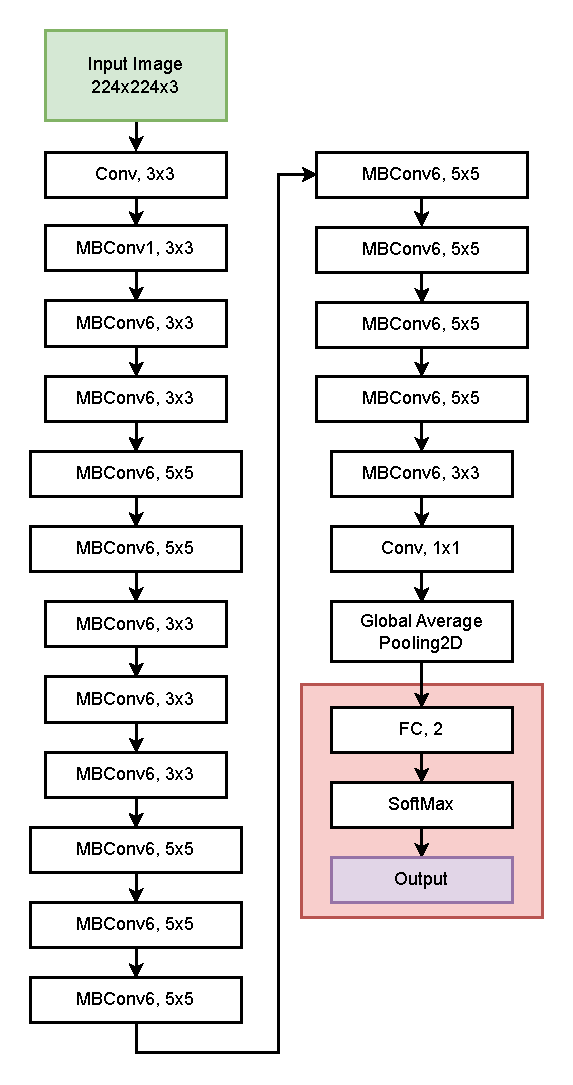
\includegraphics[width=0.5\textwidth]{graphics/images/EfficientNetB0.pdf}
	\caption{EfficientNetB0 Architecture with top layer in red box}
	\label{fig:efficientNetB0}
\end{figure}

Before utilizing the base model, three data augmentation layers are added. These are random rotation, random translation, and random flipping. These data augmentation layers are only activated during the training phase of the model and never during the testing phase. In addition to fine-tuning the pre-trained base model, a Global Average Pooling 2D layer is added, and a Dropout layer with a dropout rate of 0.3 is also added afterward. This completes the fine-tuning of the base model which is to be used in the base subnetwork of the proposed Siamese CNN model. Figure \ref{fig:pscnnsn} shows a diagram of the base subnetwork of the proposed Siamese CNN.

\begin{figure}[h]
	\centering
	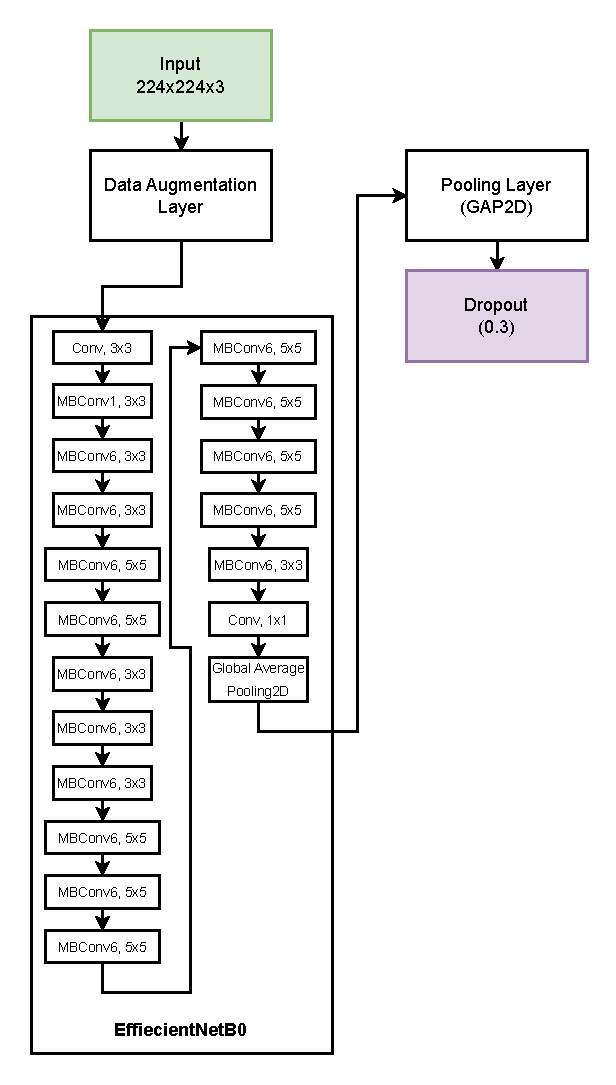
\includegraphics[width=0.5\textwidth]{graphics/images/Proposed-SCNN-Subnetwork.pdf}
	\caption{Proposed Siamese-CNN Subnetwork with pre-trained EfficientNetB0}
	\label{fig:pscnnsn}
\end{figure}

To complete the whole Siamese CNN model, two of the base subnetworks are created and then a Concat layer is instantiated with the subnetworks as inputs. Another fine-tuning is conducted after the Concat layer with an additional Dense layer of 2560 units and ReLU activation, a Global Average Pooling 2D layer, a Dropout layer with a rate of 0.4, and finally a Dense layer for the final fully connected layer with 101 units and with a SoftMax activation function. Figure \ref{fig:proposedmodel} shows an overview of the proposed Siamese CNN model. The model accepts two inputs each will be fed on each subnetwork.

\section{Dataset}
The dataset to be used in this study is the Food-101\cite{bossard-2014}. It was first used to conduct a study with regards to mining discriminative features using a novel approach called the Random Forest for machine learning \cite{bossard-2014}. Since the dataset has its ground truth, no validation set was presented when using it. Therefore, it has no predefined split like the training, validation, and evaluation. It was set as a whole, giving the user much more control in terms of utilizing it for a split. The dataset is structured into 101 classes of various foods containing a thousand image samples in JPG format in each class, producing 101000 samples in total. Each image is labeled and identified accordingly. A sample instance from the dataset is shown in \ref{fig:sampleimg}. This particular instance is labeled \textit{huevos\_rancheros/614968}. The first part of its label is the class name it is part of and the second part is its instance ID.

\begin{figure}[h]
	\centering
	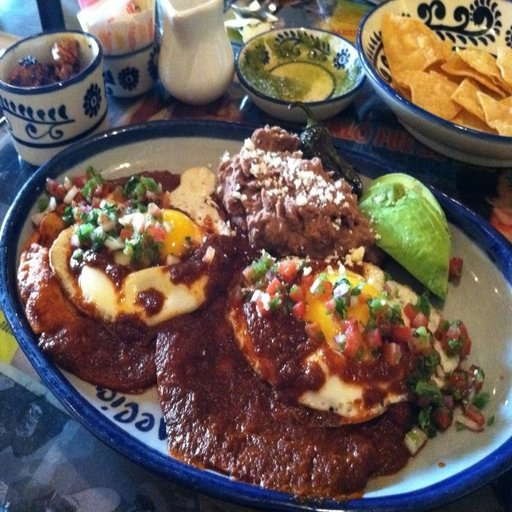
\includegraphics[width=0.5\textwidth]{graphics/images/sample_image.jpg}
	\caption{A sample instance labeled huevos\_rancheros/614968}
	\label{fig:sampleimg}
\end{figure}

The splitting of the dataset will follow the related studies \cite{pandey-2017,vijayakumari-2022,martinel-2018}. The common and most recommended way to split the dataset is by allocating samples for training, validation, and evaluation, but the studies that utilized the Food101 dataset only include the training and evaluation sets which are conducted using the 75-25 split. Since the total number of samples in the dataset is 101000, 75750 of them are allocated for the training phase and 25250 samples are to be utilized in the evaluation phase. Shown in Figure \ref{fig:dss} is the process of splitting the dataset. 

\begin{figure}[h]
	\centering
	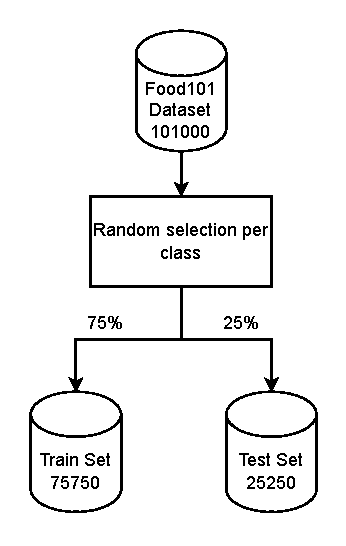
\includegraphics[width=0.5\textwidth]{graphics/images/DatasetSplit.pdf}
	\caption{Dataset Split}
	\label{fig:dss}
\end{figure}

Table \ref{tab:dataprofile} shows the data profile of the primary dataset. In the first column are the names of the classes which are the 101 food names. The second column indicates the total instances in each class which is uniform across all classes to be 1000 instances. The third column includes the number of instances in each class that will be used for the training of the model. In this case, since 75\% of each class is for training, therefore 750 instances per class are selected. The fourth column is the 25\%  remaining instances bound for the evaluation phase. The split is predetermined by the existing literature \cite{bossard-2014}. 

\begin{center}
    \begin{longtable}{|l|l|l|l|}
        \captionsetup{singlelinecheck=false, justification=raggedright, labelfont=bf}
        \caption{Food-101 Dataset Profile.} \label{tab:dataprofile} \\
        \hline
        \textbf{Class Name} & \textbf{Total Instances} & \textbf{Training Instances} & \textbf{Testing Instances} \\
        \hline
        \endfirsthead
    
        \multicolumn{4}{l}% 
        {{\bfseries \tablename\ \thetable{} -- continued from previous page}} \\ 
        \hline
        \textbf{Class Name} & \textbf{Total Instances} & \textbf{Training Instances} & \textbf{Testing Instances} \\
        \hline
        \endhead
    
        \hline \multicolumn{4}{|r|}{{Continued on next page}} \\ 
        \hline
        \endfoot
    
        \hline 
        \hline
        \endlastfoot
    
        apple pie & 1000 & 750 & 250 \\
        baby back ribs & 1000 & 750 & 250 \\
        baklava & 1000 & 750 & 250 \\
        beef carpaccio & 1000 & 750 & 250 \\
        beef tartare & 1000 & 750 & 250 \\
        beet salad & 1000 & 750 & 250 \\
        beignets & 1000 & 750 & 250 \\
        bibimbap & 1000 & 750 & 250 \\
        bread pudding & 1000 & 750 & 250 \\
        breakfast burrito & 1000 & 750 & 250 \\
        bruschetta & 1000 & 750 & 250 \\
        caesar salad & 1000 & 750 & 250 \\
        cannoli & 1000 & 750 & 250 \\
        caprese salad & 1000 & 750 & 250 \\
        carrot cake & 1000 & 750 & 250 \\
        ceviche & 1000 & 750 & 250 \\
        cheesecake & 1000 & 750 & 250 \\
        cheese plate & 1000 & 750 & 250 \\
        chicken curry & 1000 & 750 & 250 \\
        chicken quesadilla & 1000 & 750 & 250 \\
        chicken wings & 1000 & 750 & 250 \\
        chocolate cake & 1000 & 750 & 250 \\
        chocolate mousse & 1000 & 750 & 250 \\
        churros & 1000 & 750 & 250 \\
        clam chowder & 1000 & 750 & 250 \\
        club sandwich & 1000 & 750 & 250 \\
        crab cakes & 1000 & 750 & 250 \\
        creme brulee & 1000 & 750 & 250 \\
        croque madame & 1000 & 750 & 250 \\
        cup cakes & 1000 & 750 & 250 \\
        deviled eggs & 1000 & 750 & 250 \\
        donuts & 1000 & 750 & 250 \\
        dumplings & 1000 & 750 & 250 \\
        edamame & 1000 & 750 & 250 \\
        eggs benedict & 1000 & 750 & 250 \\
        escargots & 1000 & 750 & 250 \\
        falafel & 1000 & 750 & 250 \\
        filet mignon & 1000 & 750 & 250 \\
        fish and chips & 1000 & 750 & 250 \\
        foie gras & 1000 & 750 & 250 \\
        french fries & 1000 & 750 & 250 \\
        french onion soup & 1000 & 750 & 250 \\
        french toast & 1000 & 750 & 250 \\
        fried calamari & 1000 & 750 & 250 \\
        fried rice & 1000 & 750 & 250 \\
        frozen yogurt & 1000 & 750 & 250 \\
        garlic bread & 1000 & 750 & 250 \\
        gnocchi & 1000 & 750 & 250 \\
        greek salad & 1000 & 750 & 250 \\
        grilled cheese sandwich & 1000 & 750 & 250 \\
        grilled salmon & 1000 & 750 & 250 \\
        guacamole & 1000 & 750 & 250 \\
        gyoza & 1000 & 750 & 250 \\
        hamburger & 1000 & 750 & 250 \\
        hot and sour soup & 1000 & 750 & 250 \\
        hot dog & 1000 & 750 & 250 \\
        huevos rancheros & 1000 & 750 & 250 \\
        hummus & 1000 & 750 & 250 \\
        ice cream & 1000 & 750 & 250 \\
        lasagna & 1000 & 750 & 250 \\
        lobster bisque & 1000 & 750 & 250 \\
        lobster roll sandwich & 1000 & 750 & 250 \\
        macaroni and cheese & 1000 & 750 & 250 \\
        macarons & 1000 & 750 & 250 \\
        miso soup & 1000 & 750 & 250 \\
        mussels & 1000 & 750 & 250 \\
        nachos & 1000 & 750 & 250 \\
        omelette & 1000 & 750 & 250 \\
        onion rings & 1000 & 750 & 250 \\
        oysters & 1000 & 750 & 250 \\
        pad thai & 1000 & 750 & 250 \\
        paella & 1000 & 750 & 250 \\
        pancakes & 1000 & 750 & 250 \\
        panna cotta & 1000 & 750 & 250 \\
        peking duck & 1000 & 750 & 250 \\
        pho & 1000 & 750 & 250 \\
        pizza & 1000 & 750 & 250 \\
        pork chop & 1000 & 750 & 250 \\
        poutine & 1000 & 750 & 250 \\
        prime rib & 1000 & 750 & 250 \\
        pulled pork sandwich & 1000 & 750 & 250 \\
        ramen & 1000 & 750 & 250 \\
        ravioli & 1000 & 750 & 250 \\
        red velvet cake & 1000 & 750 & 250 \\
        risotto & 1000 & 750 & 250 \\
        samosa & 1000 & 750 & 250 \\
        sashimi & 1000 & 750 & 250 \\
        scallops & 1000 & 750 & 250 \\
        seaweed salad & 1000 & 750 & 250 \\
        shrimp and grits & 1000 & 750 & 250 \\
        spaghetti bolognese & 1000 & 750 & 250 \\
        spaghetti carbonara & 1000 & 750 & 250 \\
        spring rolls & 1000 & 750 & 250 \\
        steak & 1000 & 750 & 250 \\
        strawberry shortcake & 1000 & 750 & 250 \\
        sushi & 1000 & 750 & 250 \\
        tacos & 1000 & 750 & 250 \\
        takoyaki & 1000 & 750 & 250 \\
        tiramisu & 1000 & 750 & 250 \\
        tuna tartare & 1000 & 750 & 250 \\
        waffles & 1000 & 750 & 250 \\
    \end{longtable}
\end{center}

\section{Data Processing}
In engaging with deep learning, the data must be preprocessed first for the model to utilize it efficiently. Preprocessing such as rescaling, reshaping, and other preprocessing methods are selected according to what suits best to the task that the study will be focusing on.

For this study, a particular preprocessing technique is conducted called the color space conversion. Since this study focuses on the multiple color space input to image classification, it is an important part to be considered.

Before conducting a color space conversion, the image must be resized first to the required dimension for the model to process. In the proposed model, the required size should be 224 x 224. After the resizing of each instance, a single instance will be subjected to two color space conversions of choice. Given the sample instance from figure \ref{fig:sampleimg}, it was converted to 11 color spaces as presented in figure \ref{fig:colorspaces}. 

\begin{figure}[htbp]
  \centering

  \begin{subfigure}[b]{0.22\textwidth}
    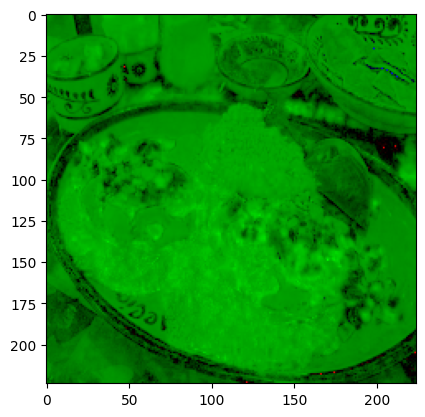
\includegraphics[width=\textwidth]{graphics/images/colorspaces/hed.png}
    \caption{HED}
    \label{fig:hed}
  \end{subfigure}
  \hfill
  \begin{subfigure}[b]{0.22\textwidth}
    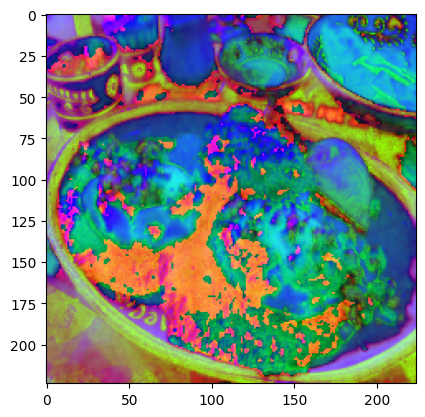
\includegraphics[width=\textwidth]{graphics/images/colorspaces/hsv.png}
    \caption{HSV}
    \label{fig:hsv}
  \end{subfigure}
  \hfill
  \begin{subfigure}[b]{0.22\textwidth}
    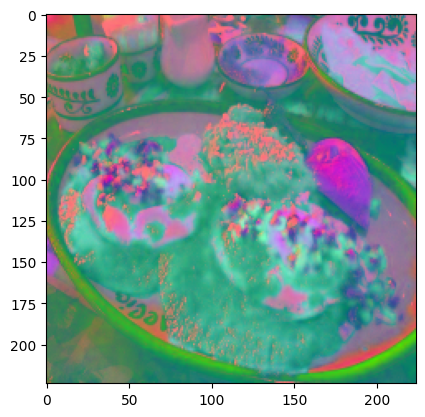
\includegraphics[width=\textwidth]{graphics/images/colorspaces/lab.png}
    \caption{LAB}
    \label{fig:lab}
  \end{subfigure}
  \hfill
  \begin{subfigure}[b]{0.22\textwidth}
    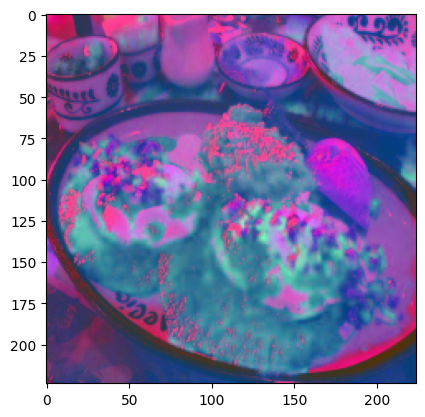
\includegraphics[width=\textwidth]{graphics/images/colorspaces/luv.png}
    \caption{LUV}
    \label{fig:luv}
  \end{subfigure}
  \hfill
  \medskip
  \begin{subfigure}[b]{0.22\textwidth}
    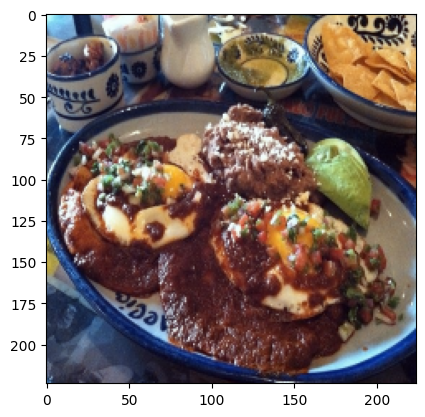
\includegraphics[width=\textwidth]{graphics/images/colorspaces/rgbcie.png}
    \caption{RGBCIE}
    \label{fig:rgbcie}
  \end{subfigure}
  \hfill
  \begin{subfigure}[b]{0.22\textwidth}
    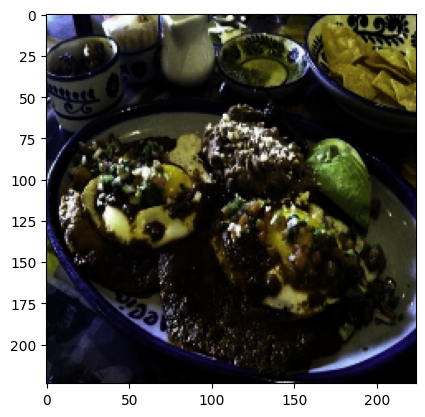
\includegraphics[width=\textwidth]{graphics/images/colorspaces/xyz.png}
    \caption{XYZ}
    \label{fig:xyz}
  \end{subfigure}
  \hfill
  \begin{subfigure}[b]{0.22\textwidth}
    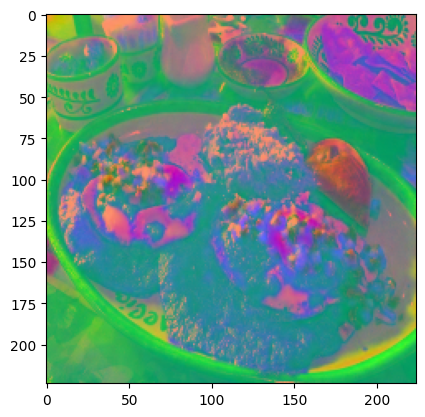
\includegraphics[width=\textwidth]{graphics/images/colorspaces/ycbcr.png}
    \caption{YCbCr}
    \label{fig:ycbcr}
  \end{subfigure}
  \hfill
  \begin{subfigure}[b]{0.22\textwidth}
    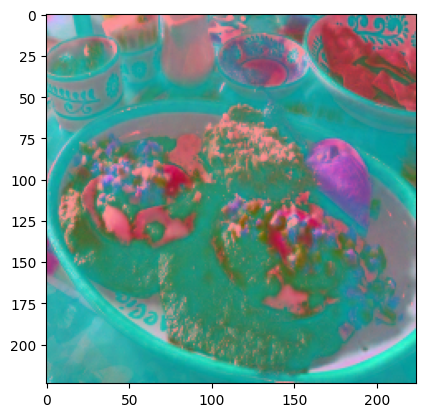
\includegraphics[width=\textwidth]{graphics/images/colorspaces/ydbdr.png}
    \caption{YDbDr}
    \label{fig:ydbdr}
  \end{subfigure}
  \hfill
  \medskip
  \begin{subfigure}[b]{0.22\textwidth}
    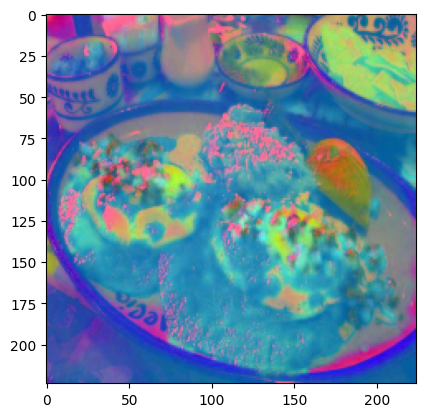
\includegraphics[width=\textwidth]{graphics/images/colorspaces/yiq.png}
    \caption{YIQ}
    \label{fig:yiq}
  \end{subfigure}
  \hfill
  \begin{subfigure}[b]{0.22\textwidth}
    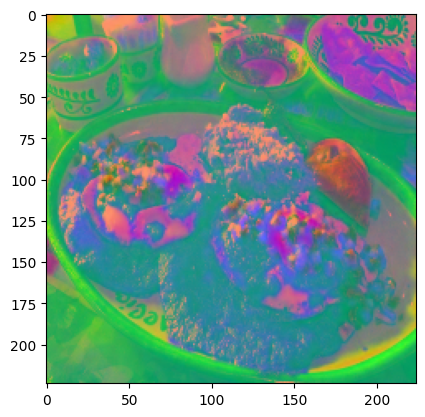
\includegraphics[width=\textwidth]{graphics/images/colorspaces/ypbpr.png}
    \caption{YPbPr}
    \label{fig:ypbpr}
  \end{subfigure}
  \hfill
  \begin{subfigure}[b]{0.22\textwidth}
    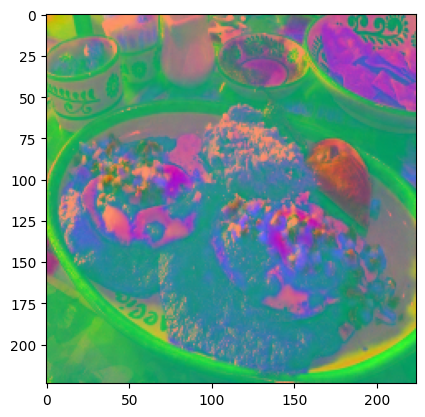
\includegraphics[width=\textwidth]{graphics/images/colorspaces/yuv.png}
    \caption{YUV}
    \label{fig:yuv}
  \end{subfigure}
 
  \caption{Images converted to color spaces}
  \label{fig:colorspaces}
\end{figure}

The conversion process also modifies the pixel values to sometimes include negative values. To address this, the function also normalizes the output image to a range [0, 255] which is necessary for the base model \cite{gangan-2022}. The image is first rescaled to the [0, 255] value range and then normalized to [0,1] to properly represent the converted image data. This will prevent the input data from being misrepresented. The normalized data is again converted to [0, 255] value range for the proposed model to process. Using the Min-Max Scaling as shown in Equation \ref{eq:mms} to normalize and rescale the image pixel data about the whole image. The output of the generic Min-Max Scaling is from [0,1] so a modification is done to achieve the [0,255] output range shown in Equation \ref{eq:mmsm}.

\begin{equation} \label{eq:mms}
X_{scaled} = \frac{X-X_{min}}{X_{max}-X_{min}}
\end{equation}
\begin{equation} \label{eq:mmsm}
X_{scaled} = \frac{X-X_{min}}{X_{max}-X_{min}} \cdot 255.0
\end{equation}

In the training phase of the model, the two converted images will be subjected to three data augmentation techniques. The random flipping, random rotation, and random translation are shown in figures \ref{fig:flipped}, \ref{fig:rotated}, and \ref{fig:translated}. Since they are in sequence, all three data augmentation techniques will result in figure \ref{fig:augmented}. Random flipping data augmentation technique is used to flip the image either horizontally, vertically, or both. Random Rotation is a data augmentation technique that rotates the image tensor to some degree. The Random Translation augmentation technique translates the image to some factor on its height and width. The use of data augmentation techniques ensures that the model sees a new instance of the sample and reduces overfitting. Some data augmentation layers are not utilized alone such as the RandomCrop layer since it produces a new shape which means an additional Reshape layer must be added to encourage more data augmentation techniques.

\begin{figure}[htbp]
  \centering

  \begin{subfigure}[b]{0.45\textwidth}
    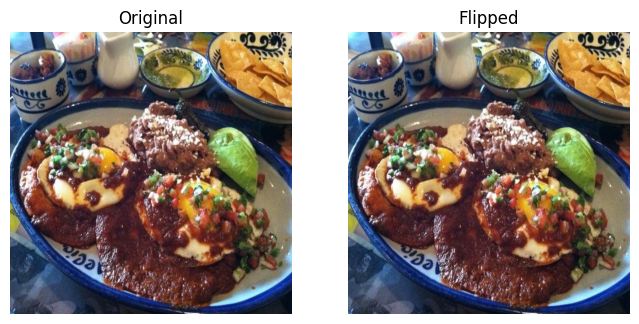
\includegraphics[width=\textwidth]{graphics/images/augmentation/flipped.png}
    \caption{Flip Augmentation}
    \label{fig:flipped}
  \end{subfigure}
  \hfill
  \begin{subfigure}[b]{0.45\textwidth}
    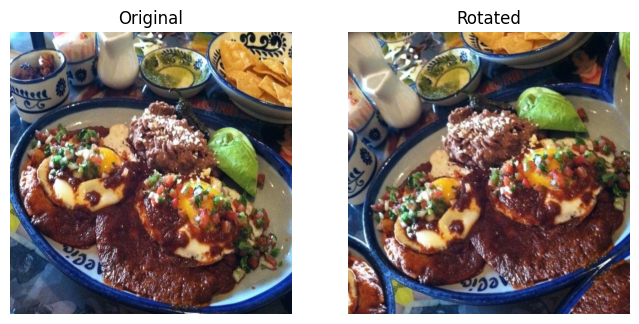
\includegraphics[width=\textwidth]{graphics/images/augmentation/rotated.png}
    \caption{Rotate Augmentation}
    \label{fig:rotated}
  \end{subfigure}
  \hfill
  \medskip
  \begin{subfigure}[b]{0.45\textwidth}
    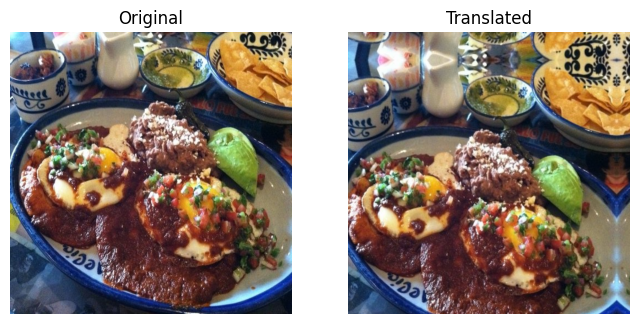
\includegraphics[width=\textwidth]{graphics/images/augmentation/translated.png}
    \caption{Translate Augmentation}
    \label{fig:translated}
  \end{subfigure}
  \hfill
  \begin{subfigure}[b]{0.45\textwidth}
    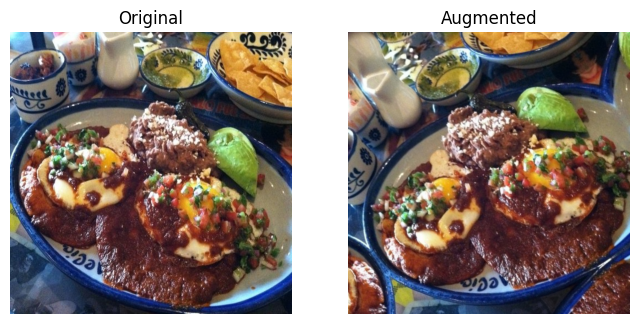
\includegraphics[width=\textwidth]{graphics/images/augmentation/augmented.png}
    \caption{The 3 augmentation}
    \label{fig:augmented}
  \end{subfigure}
  
  \caption{Images subjected to data augmentation}
  \label{fig:augmentation}
\end{figure}

\section{Model Training and Evaluation Details}
In training the model, the train split of the dataset is used. With 75\% of the total samples, the train set comprises of 75750 instances. Since each instances are converted to two color spaces, a total of 151500 instances are created but they come in pairs so there are still 75750 instances to be shuffled and batched. A batch size of 32 is used for this study and will be run on a 100-epoch limit to evaluate the baseline model. To know if the model is still learning and avoids wasting resources, 15\% of the test split is utilized per epoch to serve as a validation set.

A categorical loss function is used since this is a multiclass classification problem. This study will utilize the Categorical Cross-Entropy Loss function \cite{kumar-2018} which is defined in Equation \ref{eq:cce}. This is used to calculate the prediction disparity between the predicted value and the true value in the evaluation phase of the model. The\(p_i\) is the predicted probability of class i, which is the output of the softmax function. The \(y_i\) is the true value of the class. The summation of the true value dot product of the log of the predicted value is the standard cross-entropy formula as shown in the equation.

\begin{equation} \label{eq:cce}
CCE(p,y)= -\sum_{i=1}^{C} y_i\cdot log(p_i)
\end{equation}

An Adam optimizer is also used as an optimizer for training the model. Starting with a high learning rate of 0.01, decreasing by a factor of 0.2 when there is a plateau of validation accuracy until it reaches the lower learning rate limit of 1.0e-7. 

Callbacks are also utilized to assess the training. Specifically, the use of EarlyStopping callback to avoid wasting resources. This stops after no further improvement can be made to the validation accuracy of the training after 3 epochs. This also restores the best weight found across all runs. The ReduceLROnPlateau callback is used to dynamically adjust the learning rate of the optimizer after 1 epoch of non-improvement. This is to ensure that the model is converging efficiently. ModelCheckpoint callback is used to store the model with the best weights based on the validation accuracy of the epoch.

The final model is then used to conduct an evaluation based on the Top-5\%, and the Top-1\% benchmark. This is based on the related studies that utilized the Food101 dataset \cite{pandey-2017,vijayakumari-2022,martinel-2018}. The Top-1\% checks the probability where the predicted label matches the actual label through the highest probability in the output vector. The Top-5\% is the same as the Top-1\% but only with a wider set of choices, that is if the actual label is included in the top 5 highest probabilities.
\section{Deployment}
\begin{figure}[h]
	\centering
	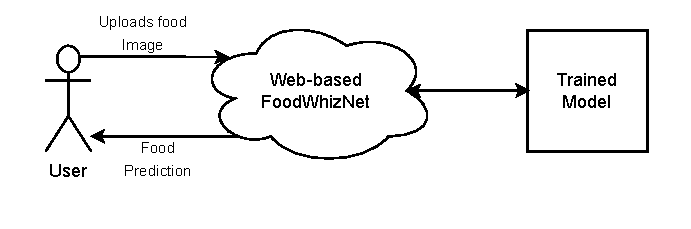
\includegraphics[width=1\textwidth]{graphics/images/deployment.pdf}
	\caption{Deployment}
	\label{fig:deploy}
\end{figure}
Shown in figure \ref{fig:deploy} is the usage of the web-based FoodWhizNet. A user is expected to upload a food image to the web application. Then, using the trained model in the backend, the image is classified accordingly and is returned to the client side of the web application and presented to the user. The best model of the study will be deployed through a web application with the front end to include CSS, HTML, and JavaScript. The backend will include the use of Flask to handle the model. A GitHub Pages will be utilized to host the web application.
\chapter{Initial Experiments and Results}
This section contains the preliminary experiments conducted on the proposed study. Specifically, this includes the two versions of the proposed model's results. The first version is the use of EfficientNetB0 and the second version is the use of the EfficientNetB1 base model. Each model has a different composition of the proposed model. The version that uses the EfficientNetB0 base model follows the initial proposed model defined in \ref{fig:initproposedmodel} we will call it Version 1 here, while the version that utilizes the EfficientNetB1 follows the \ref{fig:proposedmodel} we will call it Version 2. The reason why there are two versions is because of the improvement on the model in the later time than the conduct of some experiments. Some tests are not included here because they were done to correct the implementation of accessing of dataset and color space conversion, model improvements, consistency check for the siamese model, and transitional improvement from CNN to SCNN. 

\begin{figure}[h]
	\centering
	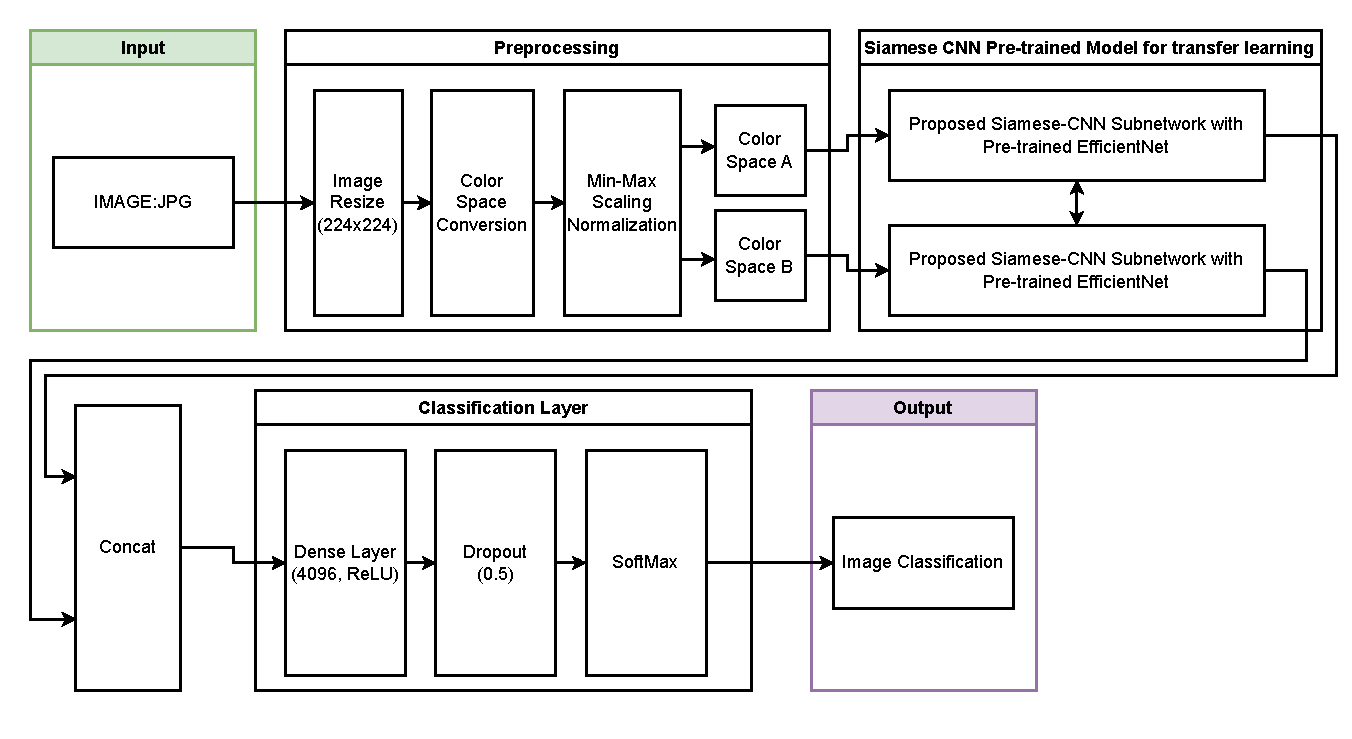
\includegraphics[width=1.0\textwidth]{graphics/images/Proposed_Model-old.pdf}
	\caption{Initial FoodWhizNet Framework}
	\label{fig:initproposedmodel}
\end{figure}

\section{Version 1 Experiments}
As mentioned earlier, Version 1 utilized the initial proposed model shown in \ref{fig:initproposedmodel} with the EfficientNetB0 base model. This particular experiment tests the best two-color space combination. Specifically, the combination of RGB and the other 10 color spaces.
\subsection{Dataset}
The conduct of this experiment includes the use of the Food101 dataset with 14 classes as identified in \cite{kaur-2023} which achieved an accuracy of 87.7\% using the EfficientNetB0 model on CNN with default RGB image. Table \ref{tab:f101c14} shows the 14 classes included in the experiment.

\begin{table}[htbp]
  \centering
  \begin{tabular}{|c|c|}
    \hline
    \textbf{Class Number} & \textbf{Class Name} \\
    \hline
    1 & apple\_pie \\
    2 & bread\_pudding \\
    3 & breakfast\_burrito \\
    4 & chicken\_wings \\
    5 & eggs\_benedicts \\
    6 & fish\_and\_chips \\
    7 & french\_fries \\
    8 & french\_onion\_soup \\
    9 & french\_toast \\
    10 & fried\_rice \\
    11 & grilled\_cheese\_sandwich \\
    12 & pizza \\
    13 & pulled\_pork\_sandwich \\
    14 & spring\_rolls \\
    \hline
  \end{tabular}
  \caption{Food 101 with 14 Classes}
  \label{tab:f101c14}
\end{table}

\subsection{Configuration}
Additional configuration includes a EarlyStopping callback with patience of 7 and monitoring the validation loss. LowerLROnPlateau callback also monitors the validation loss and a patience of 5. This experiment is a fine-tuning.
\begin{table}[htbp]
  \centering
  \begin{tabular}{|c|c|}
    \hline
    \textbf{[Hyper]parameter} & \textbf{Value} \\
    \hline
    Optimizer & Adam with initial LR of 0.01 \\
    Epochs & 100 \\
    Loss Function & Categorical Crossentropy \\
    Batch Size & 32 \\
    Shuffle Buffer Size & 1000 \\
    Shuffle Seed & 20 \\
    Augmentation Layer Seed & 42 \\
    Augmentation Layer Factors & 0.2 \\
    SubNetwork Dropout & 30\% \\
    Classification Dropout & 50\% \\
    \hline
  \end{tabular}
  \caption{Experiment Configuration of Version 1}
  \label{tab:config-v1}
\end{table}

\subsection{Results}
In this experiment of finding the best two-color space combination, RGB and XYZ stands out among the rest of the RGB combinations. Garnering a 75.51\% Top 1\% accuracy, that is 5.58\% higher than the second highest. It also achieved the top score in the Top 5\% and the lowest final loss. It has also had a promising run where it found its best weights in the 23rd epoch.
\begin{table}[h]
  \centering
  \resizebox{\textwidth}{!} & \textbf{Final Top 1\%} & \textbf{Epochs} & \textbf{Best Epoch} \\
    \hline
    RGB+LAB & 1.056701 & 94.2571 & 66.4000 &37 &27\\
    RGB+HSV & 1.120901 &92.1714 & 65.6286 & 34 & 27 \\
    RGB+HED & 1.328380 &90.1429&59.1143&31&24 \\
    RGB+LUV & 1.046469 &93.6000&67.0000&41&34 \\
   \textbf{ RGB+XYZ} & \textbf{0.816763} &\textbf{95.6571}&\textbf{75.5143}&30&23 \\
    RGB+YCbCr & 1.009330&93.4571&69.6571&41&34 \\
    RGB+YIQ &1.110264 &93.5714&65.4571&28&21 \\
    RGB+YDbDr &0.989937 &94.1714&69.8000&28&21 \\
    RGB+YPbPr & 1.057165&92.9429&67.9429&41&34\\
    RGB+YUV &1.172660 &91.4000&62.3714&28&21 \\
    \hline
  \end{tabular}
   }
  \caption{Color Space combination Results}
  \label{tab:cscr}
\end{table}

\section{Version 2 Experiment}
Version 2 utilized the new proposed model developed from model improvement to handle a large number of classes. Since the Version 1 experiment exhibits poor results on 14 classes of food 101, it might struggle to achieve even the minimum with the whole 101 classes of Food 101. It can also be observed that on \cite{kaur-2023}, they got 87.7\% for the 14 classes and the initial proposed model is far from that state-of-the-art. 

\subsection{Dataset}
The dataset used is the whole Food101 dataset \cite{bossard-2014} and profiled in table \ref{tab:dataprofile}. 

\subsection{Configuration}
The configuration includes a EarlyStopping callback with patience of 3 and monitoring the validation accuracy. LowerLROnPlateau callback also monitors the validation accuracy and a patience of 0. This experiment is a fine-tuning.

\begin{table}[htbp]
  \centering
  \begin{tabular}{|c|c|}
    \hline
    \textbf{[Hyper]parameter} & \textbf{Value} \\
    \hline
    Optimizer & Adam with initial LR of 0.01 \\
    Epochs & 100 \\
    Loss Function & Categorical Crossentropy \\
    Batch Size & 32 \\
    Shuffle Buffer Size & 1000 \\
    Shuffle Seed & 20 \\
    Augmentation Layer Seed & 42 \\
    Augmentation Layer Factors & 0.2 \\
    SubNetwork Dropout & 30\% \\
    Classification Dropout & 40\% \\
    \hline
  \end{tabular}
  \caption{Experiment Configuration of Version 2}
  \label{tab:config-v2}
\end{table}
\subsection{Results: RGB+LAB}
This version utilized the EfficientNetB1 base model. The structure of the model can be seen in \ref{fig:proposedmodel}. Ran using the RGB and LAB combination, the results are shown in figure \ref{fig:v2-accu1} for the Top 1\% accuracy of the new model with 69.93\%, \ref{fig:v2-accu5} for the Top 5\% with 90.18\%, and figure \ref{fig:v2-loss} for the final loss with 1.2020. The training took 17 epochs in total and the best weight was found on epoch 14.

\begin{figure}[htbp]
  \centering

  \begin{subfigure}[b]{0.45\textwidth}
    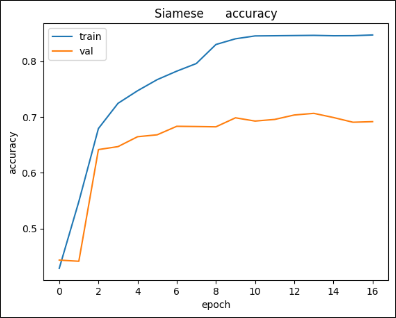
\includegraphics[width=\textwidth]{graphics/images/results/v2-accu1.png}
    \caption{Top 1 Accuracy RGB+LAB}
    \label{fig:v2-accu1}
  \end{subfigure}
  \hfill
  \begin{subfigure}[b]{0.45\textwidth}
    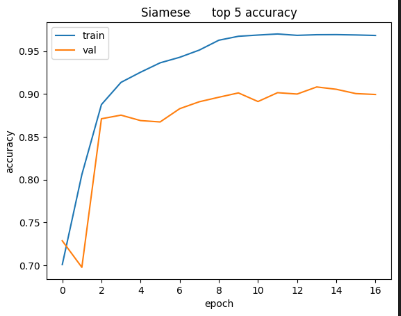
\includegraphics[width=\textwidth]{graphics/images/results/v2-accu5.png}
    \caption{Top 5 Accuracy RGB+LAB}
    \label{fig:v2-accu5}
  \end{subfigure}
  \medskip
  \begin{subfigure}[b]{0.45\textwidth}
    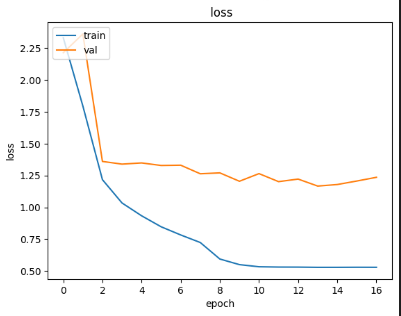
\includegraphics[width=\textwidth]{graphics/images/results/v2-loss.png}
    \caption{Final Loss RGB+LAB}
    \label{fig:v2-loss}
  \end{subfigure}
  \caption{FoodWhizNet Model Results for RGB+LAB}
  \label{fig:fwnresults}
\end{figure}

\subsection{Results: RGB+XYZ}
The same setup as the RGB+LAB experiment of Version 2, the RGB+XYZ experiment was conducted based on the initial result from the Version 1 experiment. The results are shown in figure \ref{fig:v2-accu1-rgbxyz} for the Top 1\% accuracy with 80.07\%, \ref{fig:v2-accu5-rgbxyz} for the Top 5\% with 95.04\%, and figure \ref{fig:v2-loss-rgbxyz} for the final loss with 0.7663. The training took 13 epochs in total and the best weight was found on epoch 10.

\begin{figure}[htbp]
  \centering

  \begin{subfigure}[b]{0.45\textwidth}
    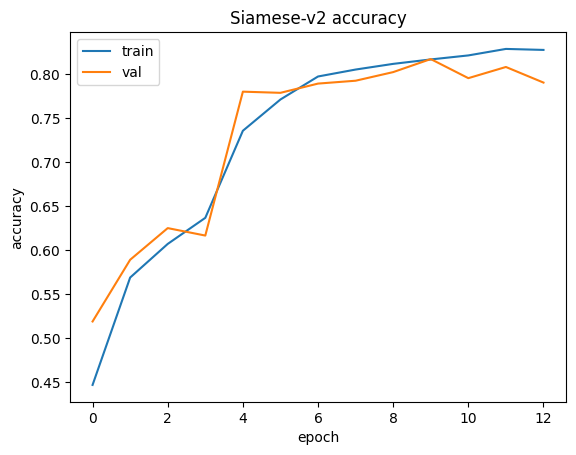
\includegraphics[width=\textwidth]{graphics/images/results/v2-accu1-rgbxyz.png}
    \caption{Top 1 Accuracy RGB+XYZ}
    \label{fig:v2-accu1-rgbxyz}
  \end{subfigure}
  \hfill
  \begin{subfigure}[b]{0.45\textwidth}
    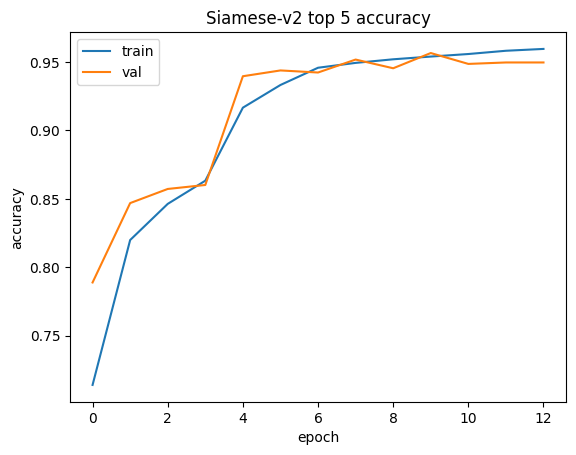
\includegraphics[width=\textwidth]{graphics/images/results/v2-accu5-rgbxyz.png}
    \caption{Top 5 Accuracy RGB+XYZ}
    \label{fig:v2-accu5-rgbxyz}
  \end{subfigure}
  \medskip
  \begin{subfigure}[b]{0.45\textwidth}
    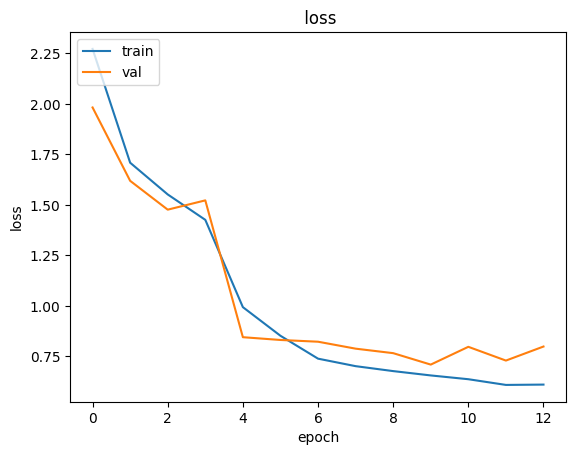
\includegraphics[width=\textwidth]{graphics/images/results/v2-loss-rgbxyz.png}
    \caption{Final Loss RGB+XYZ}
    \label{fig:v2-loss-rgbxyz}
  \end{subfigure}
  \caption{FoodWhizNet Model Results for RGB+XYZ}
  \label{fig:fwnresultsrgbxyz}
\end{figure}
\chapter{Schedule of Activities}
\begin{center}
    \begin{longtable}[l]{| p{0.18\textwidth} | p{0.18\textwidth} | p{0.18\textwidth}*{12}{| p{0.01\textwidth} }| }
    \captionsetup{singlelinecheck=false, justification=raggedright, labelfont=bf}
    \caption{Schedule of Activities.}  \\
    \hline
    \textbf{\small OBJECTIVES} & \textbf{\small TARGET ACTIVITIES} & \textbf{\small TARGET ACCOMPLISHMENTS} {\footnotesize(quantify, if possible)} & \multicolumn{12}{|c|}{\textbf{\small YEAR 1}} \\
    \hline
    % The second line, with its five years of four quarters
      & & & {\scriptsize 1} & {\scriptsize 2} & {\scriptsize 3} & {\scriptsize 4} & {\scriptsize 5} & {\scriptsize 6} & {\scriptsize 7} & {\scriptsize 8} & {\scriptsize 9} & {\scriptsize 10} & {\scriptsize 11} & {\scriptsize 12} \\
    \hline
    % using the on macro to fill in twenty cells as `on'
    {\footnotesize Objective 1} & 
    {\scriptsize To develop an alternative approach to food classification using only multiple color spaces extracted from a food image.}
    \newline &
    {\scriptsize 1. Implement an initial prototype that test the feasibility of the study using Python, Keras, and TensorFlow.} \newline
    {\scriptsize 2. Using EfficientNetB0 in building the prototype to see the performance difference between the previous studies and the current study.} \newline
    {\scriptsize 3. Using the built prototype to test the feasibility of multi-color space input performance difference between the previous studies and the current study.}
        \off[9] \on[3]\\ 
    \hline
    {\footnotesize Objective 2} & 
    {\scriptsize To conduct an ablation study on the best 2-color space input combination for the Siamese-CNN model.}
    \newline &
    {\scriptsize Given the related literature on the multi color spaces, test and validate the results and perform ablation study on the 2 best color space combination to be utilized in the study.}
        \off[9] \on[3]\\ 
    \hline
    \end{longtable}
    \newpage
    \begin{longtable}{| p{0.18\textwidth} | p{0.18\textwidth} | p{0.18\textwidth}*{12}{|p{0.01\textwidth} }| }
    \hline
    \textbf{\small OBJECTIVES} & \textbf{\small TARGET ACTIVITIES} & \textbf{\small TARGET ACCOMPLISHMENTS} {\footnotesize(quantify, if possible)} & \multicolumn{12}{|c|}{\textbf{\small YEAR 2}} \\
    \hline
    % The second line, with its five years of four quarters
      & & & {\scriptsize 1} & {\scriptsize 2} & {\scriptsize 3} & {\scriptsize 4} & {\scriptsize 5} & {\scriptsize 6} & {\scriptsize 7} & {\scriptsize 8} & {\scriptsize 9} & {\scriptsize 10} & {\scriptsize 11} & {\scriptsize 12} \\
    \hline
    % using the on macro to fill in twenty cells as `on'
    {\footnotesize Objective 3} & 
    {\scriptsize To compare the outcome of the study to the currently accepted best models in the food classification problem. } 
    \newline & 
    {\scriptsize 1. Develop the true version of the model.} \newline
    {\scriptsize 2. Perform experiments based on the methodology.} \newline
    {\scriptsize 3. Conduct a comparison and analysis on the results taken from the experiment and the previous study.} \newline
    {\scriptsize 4. Validate the feasibility of the prototype that it can outperform current best models in food classification.}
        \on[3] \off[9]\\ 
    \hline
    
    {\footnotesize Objective 4} & 
    {\scriptsize To implement a Siamese-CNN deep learning model on food classification using a web-based application.}
        \newline & 
    {\scriptsize 1. Develop the front-end of the web-based system using the HTML, CSS, and JavaScript Stack.}\newline
    {\scriptsize 2. Develop the back-end using Flask.}\newline
    {\scriptsize 3. Deploy the web-based food classification system to production.} 
        \on[4] \off[8]\\ 
    \hline
    
    \end{longtable}
\end{center}
% \chapter{Results and Discussion}
% \input{chapters/resultsdiscussion}
% \chapter{Conclusion}
% \input{chapters/conclusion}

\printbibliography[title=References]

\end{document}
